\documentclass{article}
\usepackage[utf8]{inputenc}
\usepackage[margin=1in]{geometry}
\usepackage[titletoc,title]{appendix}
\usepackage{amsmath,amsfonts,amssymb,mathtools}
\usepackage{graphicx,float}
\usepackage[ruled,vlined]{algorithm2e}
\usepackage{algorithmic}
\usepackage{minted}
\setmintedinline{breaklines}
\usemintedstyle{solarized-dark}
\usepackage{biblatex}
\addbibresource{references.bib}
\usepackage{hyperref}
\usepackage{subcaption}
\usepackage{placeins}
\usepackage{flafter}

\title{AMATH 582 Final Project}
\author{Tyrone DeSilva}
\date{February 21, 2020}

\floatname{algorithm}{Procedure}
\renewcommand{\algorithmicrequire}{\textbf{Input:}}
\renewcommand{\algorithmicensure}{\textbf{Output:}}

\begin{document}
\maketitle

\begin{abstract}
    Partial discharge is a type of fault in electric transmission lines that can
    cause damage to equipment. Detecting faults is necessary identify faulty
    equipment before failure occurs. We apply Multi-Resolution Analysis(MRA) to
    the problem of classifying faults from power line Voltage measurements.
\end{abstract}

\section{Introduction and Overview}
This data set and problem are from a data science competition \cite{vsb_data}.
The data set contains 8712 labeled training samples and 20337 unlabeled test
samples. Predictions on the unlabeled test samples are used to score
submissions. The scoring metric used in this competition is the Matthew's
correlation coefficient(MCC), which penalizes both bad recall and precision.

Each measurement consists of 3 samples, one measured from each phase of the
3-phase power delivery scheme. In both the training and test set, each signal is
labelled with it's phase. This is the breakdown of number of faults per measurement:
\begin{center}
\begin{tabular}{ |c|c|c|c| } 
\hline
\# Faults & Measurment Count \\
\hline
0 & 2710 \\ 
1 & 19 \\
2 & 19 \\
3 & 156 \\
\hline
\end{tabular}
\end{center}

This makes it pretty clear that the binary classification problem has a class
imbalance; just 6\% of the signals are faulty.
It also makes it clear that one phase displaying a fault is related
to whether the other 2 phases are also labelled faults. All 3 signals being
labelled faults occurs much more frequently than just 1 or 2 phases having faults.

Each signal has 800,000 Voltage measurements taken over 20 milliseconds. The
sampling frequency $F_s$ is 40,000,000. See Figure~\ref{fig:periodogram} and
Figure~\ref{fig:scalogram} for examples of the signals in the time domain.

In this case, there are two challenges: i) reducing the dimensionality of each
signal, ii) dealing with class imbalance. There's also the issue of encoding
information about the other phases, but for now we will treat each signal as
independent, even thought that is clearly not the case.

\section{Theoretical Background}
To preprocess our signals for classification, we used Principal Component
Analysis(PCA) and the Continuous Wavelet Transform(CWT).

PCA is a way to decompose data into the components which maximize variance, with
the aim of reducing the dimensionality of the data. This is done by finding a
diagonalization of the data. One method for PCA is diagonalizing using Singular
Value Decomposition(SVD), which is the decomposition of an arbitrary matrix $A$
into the components: $U \Sigma V^*$ where $\Sigma$ is a diagonal matrix, and
$U$, $V$ are unitary matrices. The variance of the $i$th component is
proportional to $\sigma_i^2$ where $\sigma_i$ is the $i$th diagonal element of
$\Sigma_i$. We can choose how many components of the projected matrix to keep by
calculating how many of the principal components to keep in order to account for
a given proportion of the variance.

The CWT is given as
$$
W_\psi[f](a, b) = (f, \psi_{a, b})
$$
where
$$
\psi_{a, b} = \frac{1}{\sqrt{a}}\psi(\frac{t - b}{a})
$$
$a$ and $b$ are the dilation and translation terms. The implementation of the
CWT we used to get our scalogram features are just a discretization of this
equation. Instead of $a$, $b$ being continuous we have
$$
\psi_{n, m} = \frac{1}{2^\frac{n}{v}}\psi(\frac{t}{2^\frac{n}{v}} - m F_s) \quad \mathrm{for}\quad m, n, v \in \mathbb{Z^+}
$$
CWT offers us the ability to capture both high frequency behavior with good time
resolution and lower frequency behavior with less time resolution. MRA is how we
apply the wavelet basis to get a representation of our signal at varying time
and frequency resolution.


\section{Algorithm Implementation and Development}
In addition to preprocessing our data to reduce dimensionality, we applied
Synthetic Minority Over-sampling Technique(SMOTE) to create a balanced training
set. In order to choose a model, we compared model performance on MCC score
using 5-fold cross validation. This is the algorithm we used to evaluate each model.

\begin{algorithm}
    \begin{algorithmic}
        \REQUIRE{$X$, $y$: training signals along with binary labels} 
        \ENSURE{Cross validation Score}
        \STATE $X \leftarrow \mathrm{Scalograms of} X$
        \STATE Split $X$ and $y$ into 5 folds.
        \FOR{Each fold}
            \STATE $P \leftarrow$Principal Component Vectors of training
            set
            \STATE $X \leftarrow$ Projection of all scalograms onto $P$
            \STATE Resample training folds.
            \STATE Fit model on training folds of $X$, $y$
            \STATE Score model on test fold of $X$, $y$
        \ENDFOR
        \RETURN Cross Validation Scores
    \end{algorithmic}
    \caption{Model Selection}
    \label{alg:crossval}
\end{algorithm}


\section{Computational Results}
Previously, we've used time-frequency analysis along with SVD to analyze musical
scores\cite{hw4b}. This was initially our plan for this problem, but we ran into
some short-comings of using Short Time Fourier Transform(STFT) for
time-frequency analysis. Figure~\ref{fig:periodogram} shows how STFT fails to
encode both the low and high frequency parts of the signal. We tried tuning the
STFT parameters to get some of both, but were never able to get a transform that
kept both the very high frequency and low frequency characteristics of the
signals. We wanted to capture high frequency behavior with good time resolution,
so we decided to use MRA.

Figure~\ref{fig:modes} shows some of the modes that were most significant in our
training set. It seems like the low frequency behavior is captured in the first
few modes. We needed 117 modes to capture 99.5\% of the variance, which is a big
reduction form the 15,000 dimension scalogram.

MCC score is a correlation score, so it takes on values between -1 and 1. A MCC
score of 0 is equivalent to random guessing. Our final model had an average
cross-validation MCC score of 0.210.
To get the score on the test set, we had to submit the predictions to the Kaggle
website. They have a public score(57\% of test data that is available to be
scored during the competition) and a private score(based on the held out 43\% of
the data that is held out until the competition deadline). Oddly our model did
well on the private dataset, which is the one that counts, with a MCC score of
0.216. We scored poorly on the public set, with a MCC score of 0.056.

\begin{figure}
    \centering
    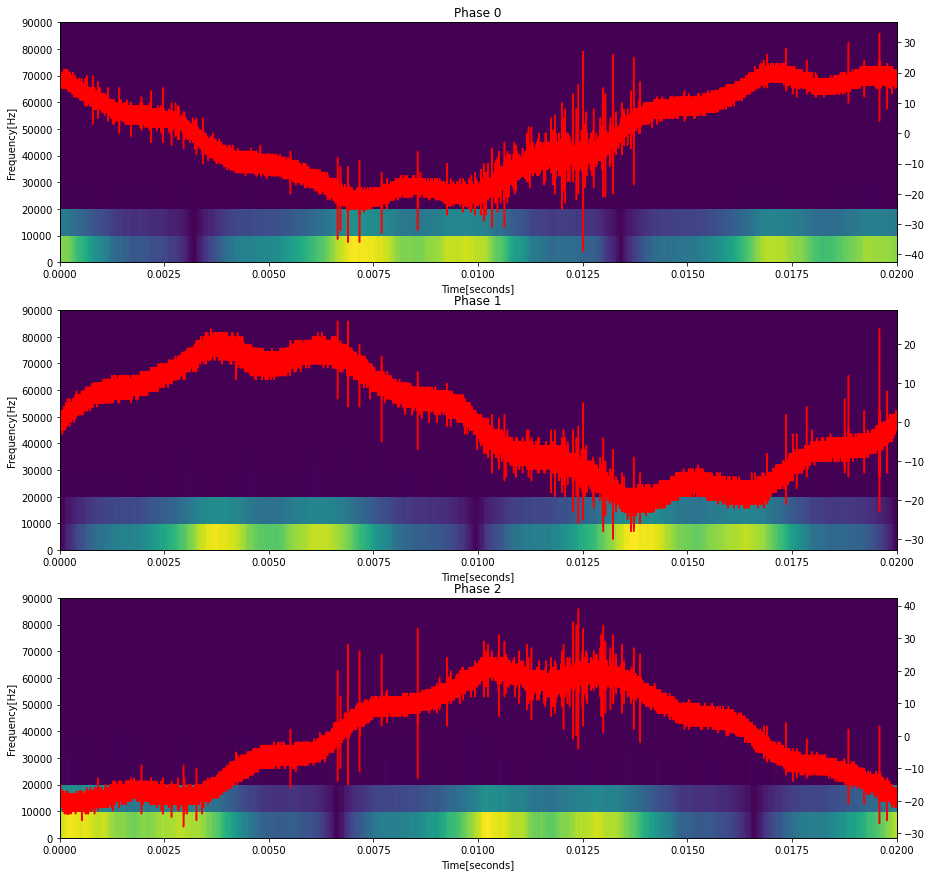
\includegraphics[width=0.8\linewidth]{stft.png}
    \caption{Periodograms for three phases along with original signals.}
    \label{fig:periodogram}
\end{figure}

\begin{figure}
    \centering
    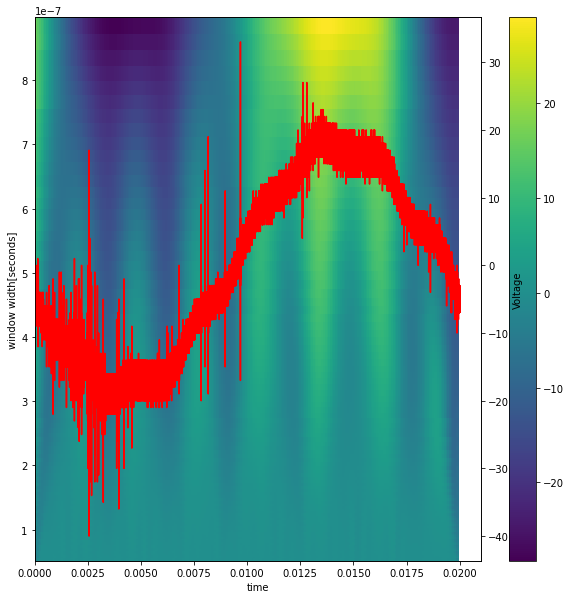
\includegraphics[width=0.6\linewidth]{cwt.png}
    \caption{Scalogram with original signal.}
    \label{fig:scalogram}
\end{figure}

\begin{figure}
    \centering
    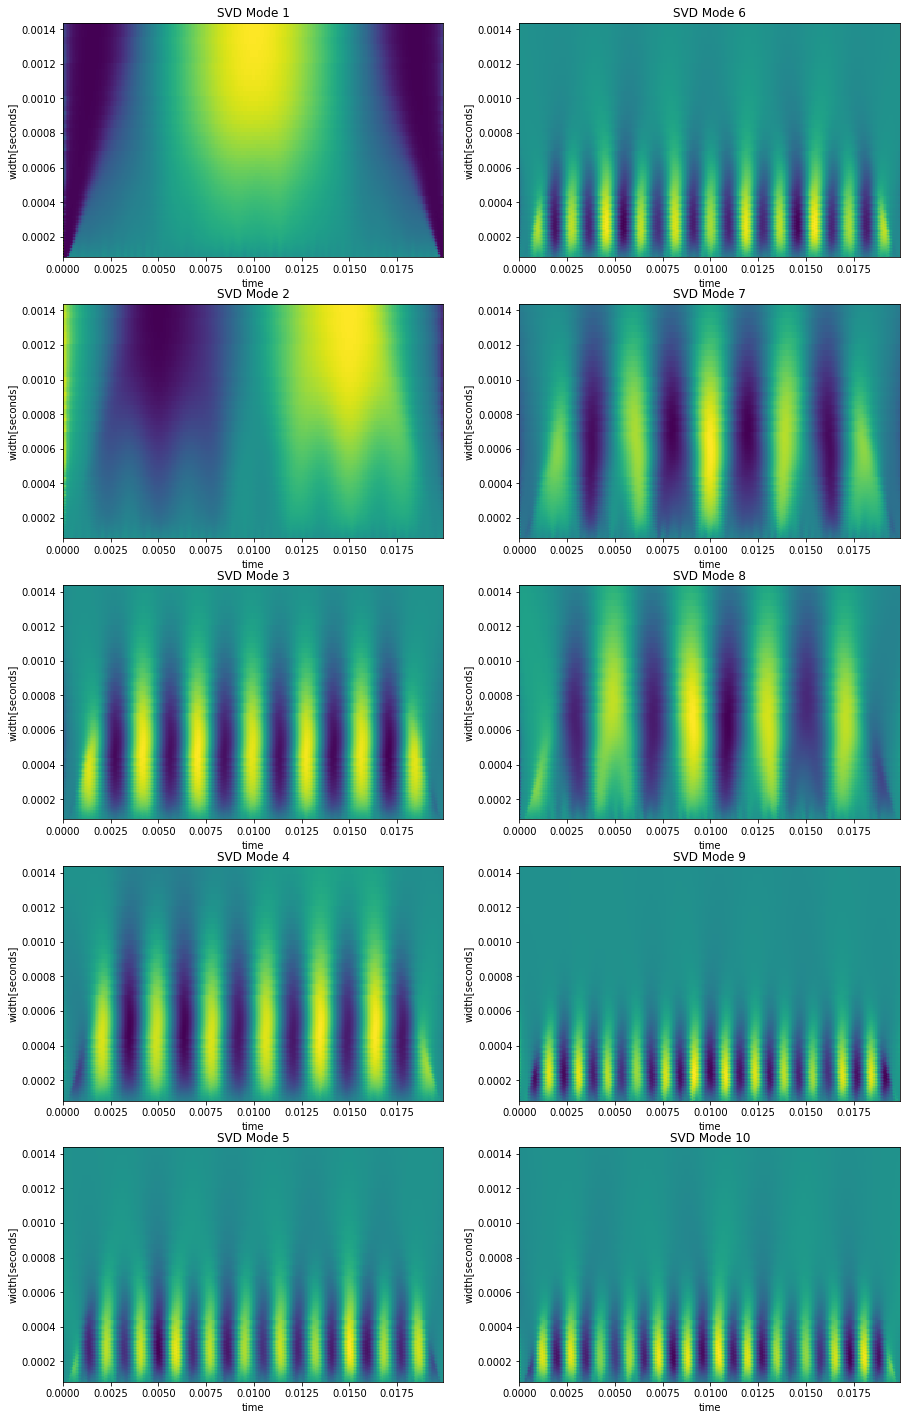
\includegraphics[width=0.8\linewidth]{pca_modes.png}
    \caption{PCA Modes}
    \label{fig:modes}
\end{figure}

\section{Summary and Conclusions}
Our final model a gradient boosting model with SMOTE. However, we used cross
validation to try a lot of different models with other sampling techniques.
In general, random undersampling was pretty close to SMOTE in terms of
performance. Without resampling, it was common for the classifier to have 0
recall and consequently score 0 MCC score as well. We also tried logistic
regression and Support Vector Classifier(SVC). Both of these under-performed the
gradient boosting model with SMOTE.

\begin{center}
\begin{tabular}{ |c|c|c|c| } 
\hline
\# Model & Cross-val MCC Score \\
\hline
Logistic Regression & 0.033 \\ 
Logistic Regression with SMOTE & 0.003 \\
Logistic Regression with Undersampling & 0.013 \\
SVC & 0.0 \\
SVC with SMOTE & 0.182 \\
Gradient Boosting & 0.085 \\
Gradient Boosting with SMOTE & 0.210 \\
Gradient Boosting with Undersampling & 0.166 \\
\hline
\end{tabular}
\end{center}


The vast majority of our time spent on this project was on preprocessing.
Initially we were planning on using the same technique as \cite{hw4b}, STFT and
PCA. It seemed like there were some high frequency, time localized behavior
happening in the signals. Without having much background knowledge on the
problem domain, it was impossible to say for certain that we didn't need good
time localization of the high frequency signals. Downsampling the signals before
applying the wavelet transform was necessary just to get everything to fit in
memory.

One alternative I was looking at, and which was mentioned in \cite{article}, is
to use the Discrete Wavelet Transform(DWT) instead of CWT. Supposedly this is
more efficient, as the CWT has a lot of redundant information. There's also more
easily available libraries to both apply DWT efficiently.

Finally, it's still unclear why performance on the public and private test sets
are so different. Test set performance is very similar to cross validation
performance. There may be pathological examples added into the public test set,
in order to throw people off who are trying to game the public test set for
information about the private test set.


\FloatBarrier
\printbibliography

\begin{appendices}
    \section{Python Functions}
        \label{sec:functions}
        \begin{itemize}
            \item \texttt{scipy.signal.cwt} Apply discretized CWT to signal.
            \item \texttt{sklearn.ensemble.GradientBoostingClassifier} Iterative
            ensemble learner for classification.
            \item \texttt{sklearn.model\_selection.cross\_validation} Fit and
            score pipeline using k-fold cross-validation.
            \item \texttt{imblearn.oversample.SMOTE} Apply SMOTE to generate
            more instances of non-majority class.
        \end{itemize}
    \section{Python Code}
        \label{sec:code}
    \subsection{preprocess.py}
        \label{subsec:preprocess}
        \inputminted{python}{preprocess.py}
    \subsection{load.py}
        \label{subsec:load}
        \inputminted{python}{load.py}
    \subsection{pca\_modes.py}
        \label{subsec:pca_modes}
        \inputminted{python}{pca_modes.py}
    \subsection{pipeline.py}
        \label{subsec:pipeline}
        \inputminted{python}{pipeline.py}
    \subsection{plots.py}
        \label{subsec:plots}
        \inputminted{python}{plots.py}

\end{appendices}
\end{document}